\begin{figure}
	\centering
	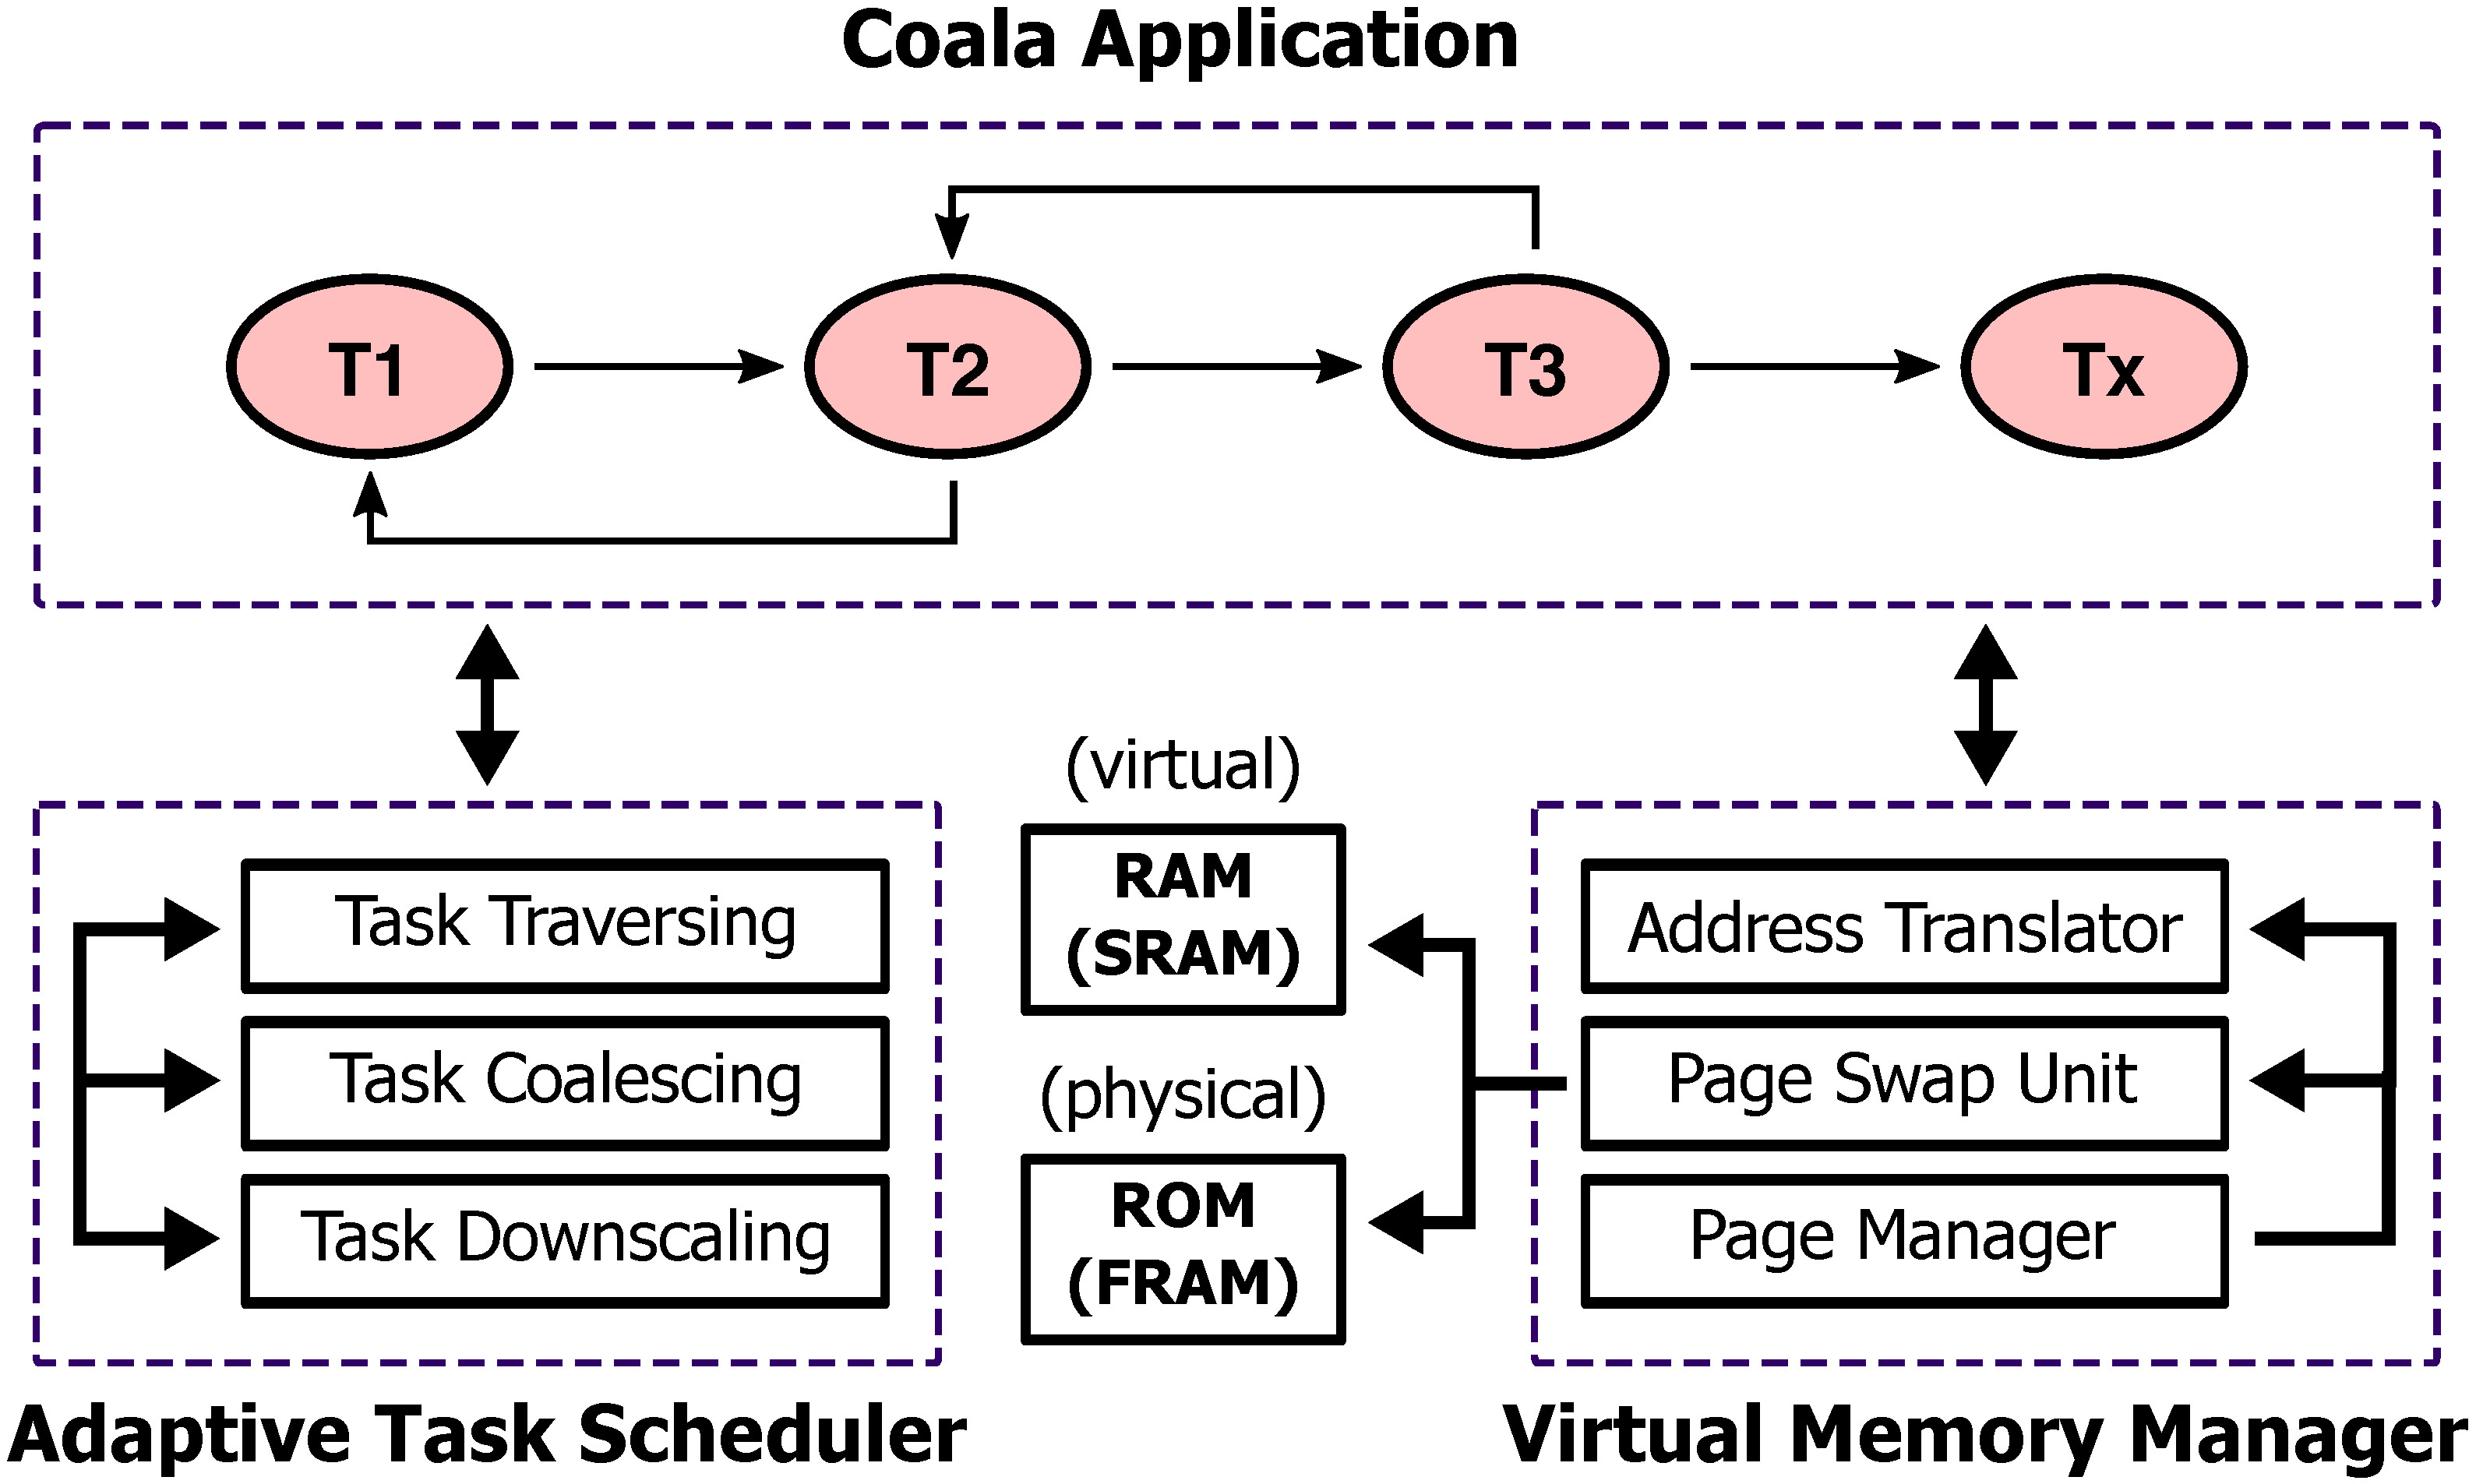
\includegraphics[width=\columnwidth]{figures/overview.pdf}
	\caption{System's top-level view. \sys is composed of two core components: \emph{Adaptive Task Scheduler} and \emph{Virtual Memory Manager}.}
	\label{fig:system_overview}
\end{figure}
%
\sys is a new programming and execution model for intermittent computing on energy-harvesting devices. \sys addresses the challenges outlined in Section~\ref{sec:background} to make task-based intermittent programs {\em programmable} and {\em efficient}. \sys accomplishes this goal with a constellation of a new programming model and runtime software system support, that supports dynamically adaptive task-based execution. Fig.~\ref{fig:system_overview} shows an overview of \sys.

\textbf{Programming and Execution Model.}  To use \sys, a programmer must convert a plain C code into tasks by encapsulating the code in a top-level set of functions, sequences the control-flow between these tasks, and annotates memory accesses that manipulate global data.
The programmer compiles their task-based code, and links to \sys runtime,
producing a \sys-enabled binary. The runtime library relies on \sys's novel
{\em virtual memory manager} and its {\em adaptive task scheduler} to adapt its execution with the energy conditions.

\textbf{Adaptive Task Scheduler(ATS).} 
\sys's adaptive task scheduler (ATS) makes \emph{energy-aware} scheduling decisions to group tasks together or split a task. By coalescing tasks \sys amortizes commit and transition costs, and by a task splitting, after repeated failures on a single task, it avoids the task non-termination problem. The scheduler uses its recent execution history---no hardware dependency---as a metric to estimate energy availability and eventually to decide on the dynamic task size. 

\textbf{Virtual Memory Manager (VMM).} \sys is able to efficiently coalesce
tasks because of its efficient virtual memory manager (VMM).
the VMM privatizes a group of memory pages demanded by a coalesced task, and limits an application access only to the fast volatile memory. It persists all pages modifications in non-volatile memory on a coalesced task transition. Section~\ref{sec:memory_virtulaization} provides details of VMM.
